\documentclass[10pt,letterpaper]{article}
\usepackage[utf8]{inputenc}
\usepackage[T1]{fontenc}
\usepackage[spanish]{babel}
\usepackage{listings}
\usepackage{graphicx}
\graphicspath{{imagenes/}} %paqute para que pueda jalar mi imagen del diagrama
\usepackage{float}
\usepackage{comment}
\usepackage{tabularx}
\usepackage{float}
\usepackage{float} %para que no se mueve de lugar mis imagenes
% Preámbulo

\title{Documentacion de un Sistema de Gestion para una Tienda Online}
\author{Beatriz Garcia Lopez }
\date{\today}

\usepackage{xcolor}

\definecolor{codegreen}{rgb}{0,0.6,0}
\definecolor{codegray}{rgb}{0.5,0.5,0.5}
\definecolor{codepurple}{rgb}{0.58,0,0.82}
\definecolor{backcolour}{rgb}{0.95,0.95,0.92}

\lstdefinestyle{mystyle}{
    backgroundcolor=\color{backcolour},   
    commentstyle=\color{codegreen},
    keywordstyle=\color{magenta},
    numberstyle=\tiny\color{codegray},
    stringstyle=\color{codepurple},
    basicstyle=\ttfamily\footnotesize,
    breakatwhitespace=false,         
    breaklines=true,                 
    captionpos=b,                    
    keepspaces=true,                 
    numbers=left,                    
    numbersep=5pt,                  
    showspaces=false,                
    showstringspaces=false,
    showtabs=false,                  
    tabsize=2
}
\lstset{style=mystyle}

\begin{document}
\maketitle




\section{Introducción}
Se nos ha solicitado diseñar y construir la base de datos completa para gestionar las operaciones de una tienda online,
 asegurando que la información de productos, clientes y ventas esté organizada y protegida.
% En "2. Descripción del problema":
\section{Descripción del problema}
Lo que hace este sistema es resolver el desorden en el inventario y las ventas.
 Permite registrar qué compró cada cliente, saber exactamente cuántos productos 
 quedan disponibles y evitar que se vendan artículos agotados.
\section{Análisis y Diseño}
En este apartado vamos a estructurar un poco las tablas y implementar un DER(Diagrama Entidad-Relacion) utilizando la página "Draw.io"
\begin{table}[h]%para que lo ponga justo abajo de "Analisis"
    \begin{tabular}{| c |p{9cm} |} % esto sirve para dar un salto de linea para que no se siga de largo en LaTeX
        \hline
        TABLAS & ¿QUE ORGANIZA? \\
        \hline
        Categorias                 & Organiza los productos en 5 categorias diferentes
                                      (telefonos, laptops, accesorios, tablets y relojes inteligentes)\\ \hline
        
        Reseñas                    & Registra las reseñas de los productos y el ranking del mismo, el cual se evalua de
                                      1 a 5 estrellas, siendo 1 = muy malo y 5 = excelente. Un detalle importante es que
                                      las reseñas solo podran ser realizadas por clientes que hayan comprado un producto,
                                      sin importar la categoria del mismo.\\ \hline

        Pedidos                    & Especifica los detalles especificos del producto; como fecha de pedido y el estado
                                      del mismo (Enviado, Pendiente y Entregado).\\ \hline
        
        Detalles del Pedido        & Guarda los datos especificos del pedido como por ejemplo
                                      la cantidad (¿cuantos productos se van a enviar?) y el precio unitario del producto.\\ \hline
        
        Productos                  & Esta tabla es la mas importante ya que desde aqui vamos a poder gestionar todas las demas tablas.
                                      Es como un "gestor que se conecta con todo lo demas". De igual manera, aqui tenemos el nombre, descripcion, precio y stock de todos los
                                      productos disponibles al momento.\\ \hline

        Clientes                   & En esta tabla esta toda la informacion personal del cliente como por ejemplo nombre, correo, telefono y direccion.\\ \hline
    

    \end{tabular}
    \clearpage

    A continuacion tenemos un diagrama ER explicando de mejor manera la tabla
\end{table}
\subsection{Diagrama Entidad-Relacion}
\begin{figure}[H]
    \centering
    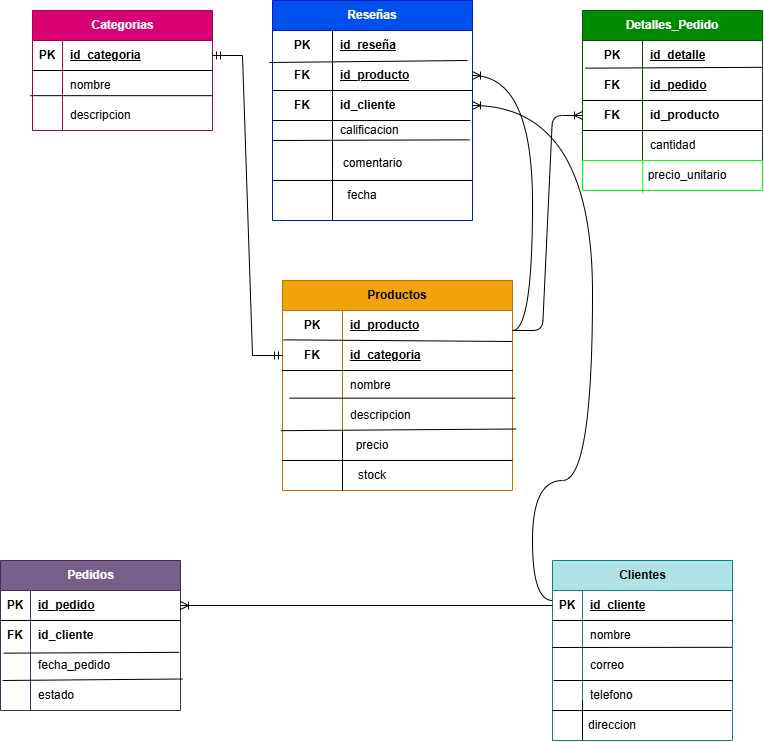
\includegraphics[width=0.7\textwidth]{imagenes/DER.png}
    \caption{DER de la Base de Datos}
    \label{fig:diagrama_er}
\end{figure}
\clearpage
\subsection{Esquema en tercera forma normal (3NF), con justificación de normalización.}
 \textbf{Primera Forma Normal (1NF)}: Todas las tablas tienen datos atómicos. Esto significa que no tenemos listas con datos mezclados  
en una sola celda; cada campo guarda un solo dato. Por ejemplo, en la tabla \textbf{Clientes}, el nombre, correo y teléfono están 
separados en sus propios campos, en lugar de tener un solo campo saturado de "datos de contacto".

\textbf{Segunda Forma Normal (2NF)}: Todos los datos de una tabla dependen por completo de su llave principal(PK).
    Un excelente ejemplo del diseño es la tabla \textbf{Detalles\_Pedido}: la cantidad de productos comprados 
    depende exactamente de esa línea de compra en específico (id\_detalle), no solo del pedido ni del producto por sí solos.

\textbf{Tercera Forma Normal (3NF)}: Ningún dato depende de otro que no sea la llave principal. Tenemos dos ejemplos:
\begin{itemize}
    \item En la tabla \textbf{Pedidos}, no pusimos el nombre del cliente dentro de la tabla, porque el nombre depende del cliente (por eso tiene su propia tabla),
    no del pedido en sí. Solo los unimos con la llave foránea "id\_cliente".
\end{itemize}
 
En la tabla Productos, no fue necesario escribir el nombre o la descripción de la categoría. Solo usamos id\_categoria. Así, si la categoría cambia de nombre,
 se actualiza en su propia tabla y no crea inconsistencias en los productos.

\subsection{Identificación de Claves}
A continuación se detallan las claves primarias, foráneas y candidatas de cada entidad dentro del modelo relacional del proyecto:

\subsubsection*{Claves Primarias (PK)}
Las claves primarias seleccionadas actúan como identificadores únicos e irrepetibles para cada registro dentro de su respectiva tabla:
\begin{itemize}
    \item \textbf{Categorias:} \texttt{id\_categoria}
    \item \textbf{Productos:} \texttt{id\_producto}
    \item \textbf{Clientes:} \texttt{id\_cliente}
    \item \textbf{Pedidos:} \texttt{id\_pedido}
    \item \textbf{Detalles\_Pedido:} \texttt{id\_detalle}
    \item \textbf{Reseñas:} \texttt{id\_reseña}
\end{itemize}

\subsubsection*{Llaves Foráneas (FK)}
Las llaves foráneas establecen la integridad referencial y las relaciones entre las entidades del sistema:
\begin{itemize}
    \item \textbf{Productos:} \texttt{id\_categoria} (referencia a la tabla \texttt{Categorias})
    \item \textbf{Pedidos:} \texttt{id\_cliente} (referencia a la tabla \texttt{Clientes})
    \item \textbf{Detalles\_Pedido:} \texttt{id\_pedido} (referencia a la tabla \texttt{Pedidos}) y \texttt{id\_producto} (referencia a la tabla \texttt{Productos})
    \item \textbf{Reseñas:} \texttt{id\_producto} (referencia a la tabla \texttt{Productos}) y \texttt{id\_cliente} (referencia a la tabla \texttt{Clientes})
\end{itemize}

\subsubsection*{Llaves Candidatas}
Las llaves candidatas son aquellos atributos que también poseen la cualidad de unicidad y podrían funcionar como identificadores principales, aunque se haya optado por un ID numérico por eficiencia:
\begin{itemize}
    \item \textbf{Clientes:} El atributo \texttt{correo} es una llave candidata fuerte, ya que en el sistema de ventas no deberían existir dos clientes registrados con la misma dirección de correo electrónico.
    \item \textbf{Categorias:} El atributo \texttt{nombre} funciona como llave candidata, ya que no tendría sentido comercial tener dos categorías llamadas exactamente igual.
\end{itemize}

\section{Implementacion de la Base de Datos}
En esta sección se presenta el script correspondiente a la creación del esquema relacional, la definición de llaves primarias y foráneas,
 así como las restricciones de integridad y la creación de índices para optimizar las consultas. Finalmente, se incluye el código utilizado 
 para poblar la base de datos con registros de prueba

\begin{lstlisting}[language=SQL, caption=Creación de Base de Datos]
-- 1. Crear esquema y limpiar versiones viejas
CREATE SCHEMA IF NOT EXISTS proyecto_final_bd;
USE proyecto_final_bd;
DROP TABLE IF EXISTS Resenas, Detalles_Pedido, Pedidos, Productos, Clientes, Categorias;

-- 2. Crear las tablas principales
CREATE TABLE Categorias (id_categoria INT PRIMARY KEY, nombre VARCHAR(50), descripcion VARCHAR(200));
CREATE TABLE Clientes (id_cliente INT PRIMARY KEY, nombre VARCHAR(100), correo VARCHAR(100) UNIQUE, telefono VARCHAR(20), direccion VARCHAR(200));
CREATE TABLE Productos (id_producto INT PRIMARY KEY, nombre VARCHAR(100), descripcion VARCHAR(200), precio DECIMAL(10,2), stock INT CHECK (stock >= 0), id_categoria INT, FOREIGN KEY (id_categoria) REFERENCES Categorias(id_categoria));
CREATE TABLE Pedidos (id_pedido INT PRIMARY KEY, id_cliente INT, fecha_pedido DATE, estado VARCHAR(20), FOREIGN KEY (id_cliente) REFERENCES Clientes(id_cliente));
CREATE TABLE Detalles_Pedido (id_detalle INT PRIMARY KEY, id_pedido INT, id_producto INT, cantidad INT, precio_unitario DECIMAL(10,2), FOREIGN KEY (id_pedido) REFERENCES Pedidos(id_pedido), FOREIGN KEY (id_producto) REFERENCES Productos(id_producto));
CREATE TABLE Resenas (id_resena INT PRIMARY KEY, id_producto INT, id_cliente INT, calificacion INT, comentario VARCHAR(255), fecha DATE, FOREIGN KEY (id_producto) REFERENCES Productos(id_producto), FOREIGN KEY (id_cliente) REFERENCES Clientes(id_cliente));

-- 3. Crear indices para agilizar busquedas
CREATE INDEX idx_producto_nombre ON Productos(nombre);
CREATE INDEX idx_producto_categoria ON Productos(id_categoria);
CREATE INDEX idx_pedido_cliente ON Pedidos(id_cliente);

-- 4. Insertar datos (Muestra representativa)
INSERT IGNORE INTO Categorias (id_categoria, nombre, descripcion) VALUES (1, 'Laptops', 'Computadoras portatiles');
INSERT IGNORE INTO Clientes (id_cliente, nombre, correo, telefono, direccion) VALUES (1, 'Juan Perez', 'juan@email.com', '5551112222', 'Calle 1');
\end{lstlisting}

\begin{figure}[H]
    \centering
    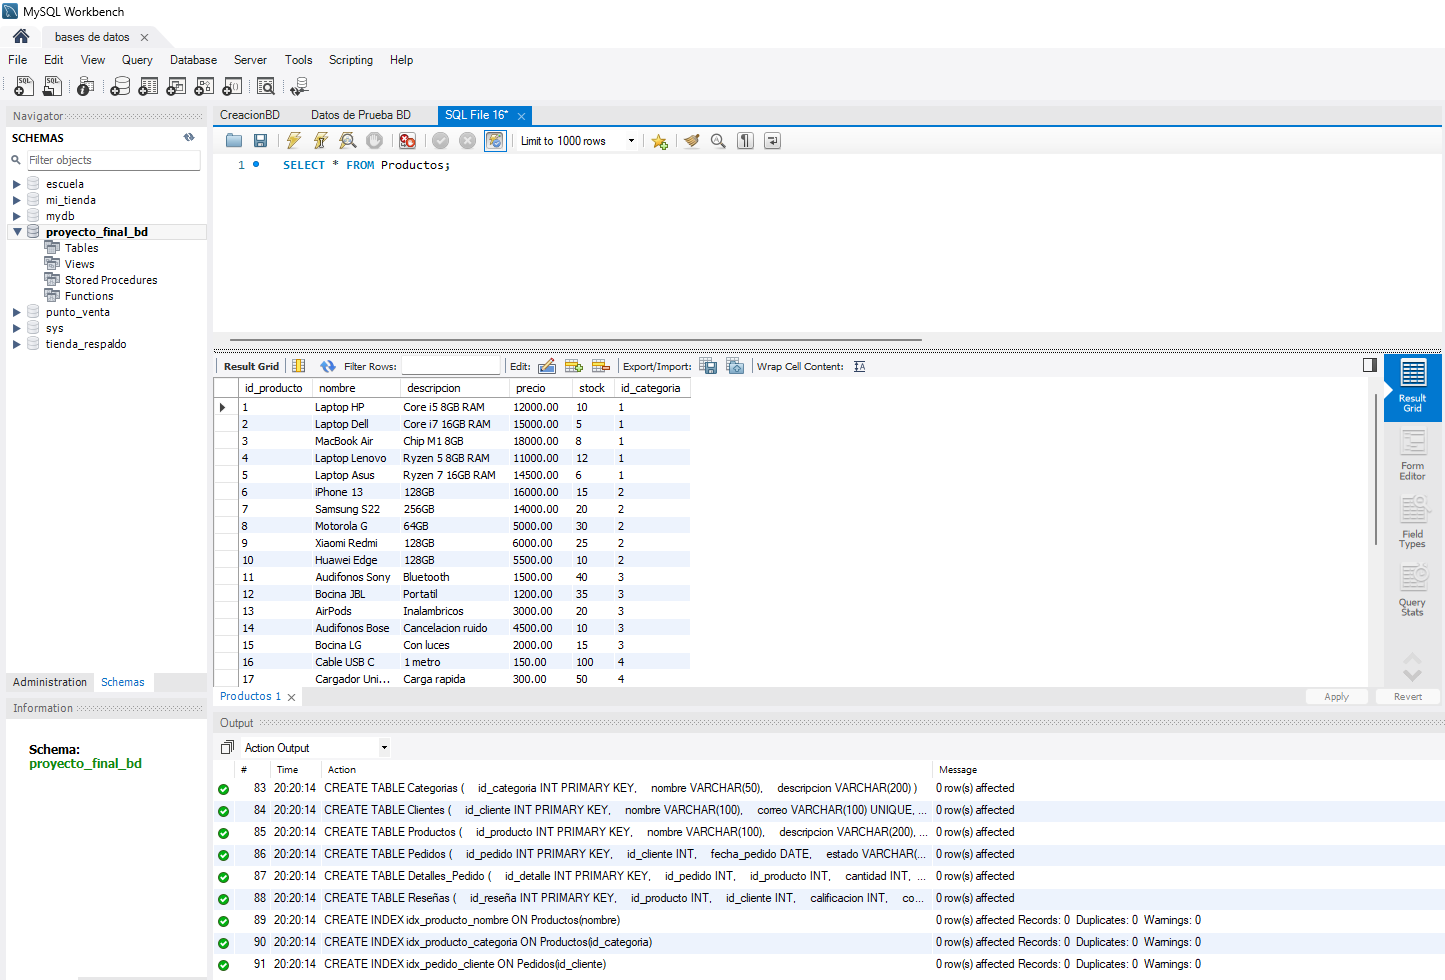
\includegraphics[width=0.7\textwidth]{Preuba 1 Poblar la BD.png}
    \label{fig:prueba 1  poblacion de la BD }
\end{figure}
\clearpage

% --- SECCIÓN 5 ---
\section{Consultas y Procedimientos Almacenados}
\begin{lstlisting}[language=SQL, caption=Lógica de Negocio]
-- Consultar clientes con pedidos pendientes
SELECT c.nombre, COUNT(p.id_pedido) AS total_pendientes
FROM Clientes c JOIN Pedidos p ON c.id_cliente = p.id_cliente
WHERE p.estado = 'Pendiente' GROUP BY c.id_cliente;

-- Procedimiento: Registrar pedido limitando a 5 pendientes
DROP PROCEDURE IF EXISTS sp_registrar_pedido;
DELIMITER //
CREATE PROCEDURE sp_registrar_pedido(IN p_cliente INT)
BEGIN
    DECLARE v_pendientes INT;
    DECLARE v_id INT;
    SELECT COUNT(*) INTO v_pendientes FROM Pedidos WHERE id_cliente = p_cliente AND estado = 'Pendiente';
    
    IF v_pendientes < 5 THEN
        SELECT IFNULL(MAX(id_pedido), 0) + 1 INTO v_id FROM Pedidos;
        INSERT INTO Pedidos (id_pedido, id_cliente, fecha_pedido, estado) VALUES (v_id, p_cliente, CURDATE(), 'Pendiente');
    ELSE
        SIGNAL SQLSTATE '45000' SET MESSAGE_TEXT = 'Limite alcanzado';
    END IF;
END //
DELIMITER ;
\end{lstlisting}
\begin{figure}[H]
    \centering
    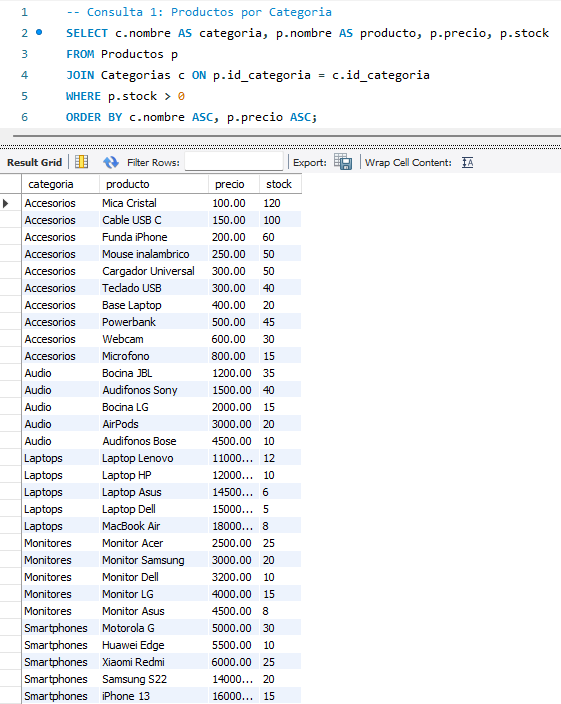
\includegraphics[width=0.7\textwidth]{Consulta1 .png}
    \caption{Resultado de la consulta 1: Productos por categoría.}
    \label{fig:Consulta 1}
\end{figure}

\begin{figure}[H]
    \centering
    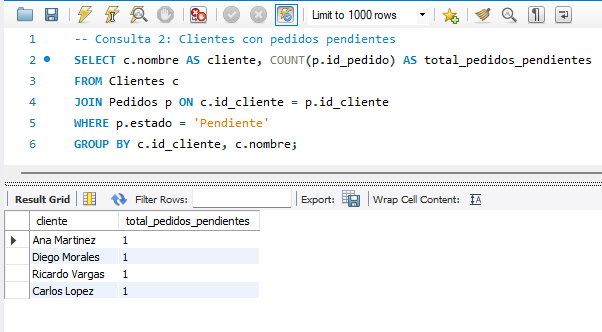
\includegraphics[width=0.7\textwidth]{Consulta 2.png}
    \caption{Resultado de la consulta 2: Clientes con pedidos pendientes.}
    \label{fig:Consulta 2}
\end{figure}

\begin{figure}[H]
    \centering
    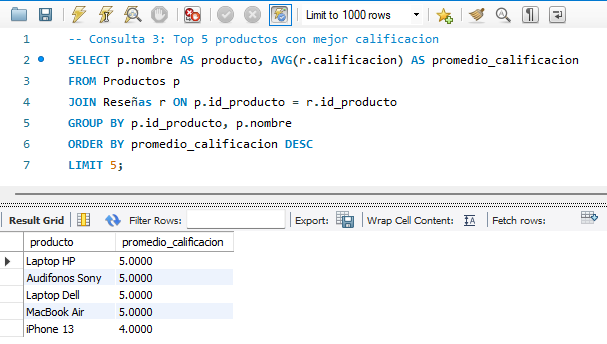
\includegraphics[width=0.7\textwidth]{Consulta3.png}
    \caption{Resultado de la consulta 3: Top 5 productos mejor calificados.}
    \label{fig:Consulta 3}
\end{figure}


% --- SECCIÓN 6 ---
\section{Validación y Optimización}
Para comprobar que la lógica funciona, ejecutamos el procedimiento de reporte de stock mediante el comando \texttt{CALL}, obteniendo los datos esperados.
\begin{figure}[H]
    \centering
    % AQUÍ VA LA IMAGEN DEL CALL (La que tiene 1 sola fila con Laptop Asus)
    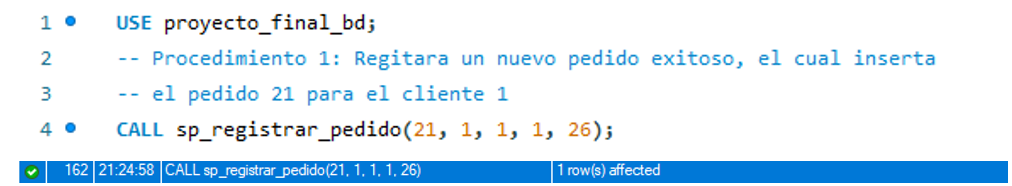
\includegraphics[width=0.7\textwidth]{Procedimiento1.png}
    \caption{Ejecución exitosa del procedimiento almacenado (Reporte de stock).}
\end{figure}

Para validar la optimización, usamos la instrucción \texttt{EXPLAIN}. La base de datos utilizó correctamente nuestro índice \texttt{idx\_producto\_nombre}, encontrando la Laptop en una sola lectura (\textbf{rows = 1}).
\begin{figure}[H]
    \centering
    % AQUÍ VA LA IMAGEN DEL EXPLAIN (La tabla larga con muchos datos)
    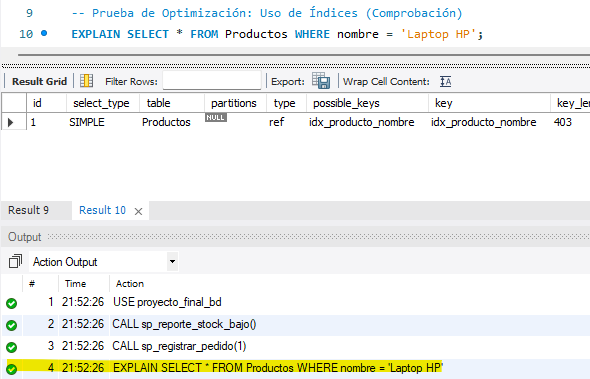
\includegraphics[width=0.7\textwidth]{OP_VAL3.png}
    \caption{Uso de índices en búsqueda rápida.}
\end{figure}


\section{Errores y Correcciones}
\begin{table}[H]
    \centering
    \begin{tabularx}{\textwidth}{|l|X|X|}
    \hline
    \textbf{Problema} & \textbf{Causa} & \textbf{Solución} \\ \hline
    Error 1054: Unknown column & Nombres de llaves foráneas automáticos y confusos. & Estandarizar la creación de tablas con nombres limpios (ej. \texttt{id\_cliente}). \\ \hline
    Warning 1366 & Insertar datos sin especificar el orden de las columnas. & Declarar las columnas explícitamente en cada inserción. \\ \hline
    Error 1452: Foreign key fails & Guardar detalles de un pedido antes que el producto. & Respetar la jerarquía insertando primero los datos padre (categorías, productos). \\ \hline
    Error 1318: Incorrect arguments & Actualizar un procedimiento sin borrar el viejo de la memoria. & Usar \texttt{DROP PROCEDURE IF EXISTS} al inicio. \\ \hline
    \end{tabularx}
    \caption{Resolución de problemas técnicos.}
\end{table}

% --- SECCIÓN 8 ---
\section{Conclusión}
Desarrollar este sistema me permitió entender que una base de datos no es solo guardar información, sino conectarla con lógica real. Aprendí a estructurar las tablas usando normalización, a proteger la información con restricciones y a automatizar procesos con procedimientos almacenados, logrando un proyecto totalmente funcional y libre de errores.

% --- SECCIÓN 9 ---
\section{Material de Apoyo Consultado}
\begin{itemize}
    \item Monroy, G. (2026). \textit{Procedimientos Almacenados, Vistas y Triggers en MySQL}. Material de clase.
    \item Parzibyte - programador. (s. f.). https://parzibyte.me/
    \item Ivan. (2011, 25 diciembre). Crear BD en MySQL Workbench: Guía paso a paso para principiantes 
     MySQL YA. Mysql YA. https://mysqlya.com.ar/tutoriales/crear-bd-en-mysql-workbench/
    \item Andrés, J. (s. f.). DISEÑO y CREACIÓN DE BASE DE DATOS CON MYSQL WORKBENCH (BD INVENTARIO).
     https://base-de-datos-online.blogspot.com/2016/01/diseno-y-creacion-de-base-de-datos-con.html
    \item Parzibyte. (2021, 20 enero). MySQL - Inner join con count usando subconsulta. 
    Parzibyte. https://parzibyte.me/blog/posts/mysql-inner-join-count-subconsulta/
\end{itemize}



\end{document}